\documentclass[aspectratio=169,11pt]{beamer}

\usetheme{metropolis}
\usecolortheme{seahorse}
\usefonttheme{professionalfonts}

\usepackage[spanish,es-tabla]{babel}
\usepackage[utf8]{inputenc}
\usepackage[T1]{fontenc}
\usepackage{amsmath,amssymb}
\usepackage{siunitx}
\usepackage{booktabs}
\usepackage{graphicx}
\usepackage{circuitikz}
\usepackage{tikz}
\usepackage{adjustbox}
\usepackage{xcolor}
\usepackage{multicol}
\usetikzlibrary{positioning,arrows.meta,shapes.geometric,calc}

\graphicspath{{figuras/}}
\sisetup{output-decimal-marker={,}, per-mode=symbol}

\definecolor{tcblue}{RGB}{0,75,135}
\definecolor{tcorange}{RGB}{230,120,20}
\definecolor{tcgray}{RGB}{245,246,248}
\setbeamercolor{frametitle}{fg=white,bg=tcblue}
\setbeamercolor{progress bar}{fg=tcorange,bg=tcgray}
\setbeamercolor{alerted text}{fg=tcorange}
\setbeamertemplate{frame numbering}[fraction]
\setbeamertemplate{navigation symbols}{}

\newcommand{\figpath}{figuras/}
\newcommand{\Hpb}{H_{PB}}
\newcommand{\Hpa}{H_{PA}}
\newcommand{\smallnote}[1]{\vspace{0.3em}{\scriptsize\color{gray!70!black}#1}}

\title{Trabajo Práctico Final}
\subtitle{Python, LTspice IV y Altium Designer}
\author{Grupo 8\\Mariano Cáceres Smoler · Tomás Francisco Castro\\Jorge López Arauz · Lucca Nehuen Yaggi}
\institute{Teoría de Circuitos I -- ITBA}
\date{2026}

\begin{document}

% -----------------------------------------------------------------
\begin{frame}[plain]
    \titlepage
\end{frame}

\begin{frame}{Objetivo de la presentación}
    \begin{columns}[T,onlytextwidth]
        \column{0.52\textwidth}
        \begin{block}{Qué se desarrolló}
        \begin{itemize}
            \item GUI en Python para CSV de osciloscopio, simulación y Bode.
            \item Simulación y medición de transitorios RLC.
            \item Análisis de filtros RLC de segundo orden.
            \item Diseño de un filtro pasabanda para voz humana e implementación en PCB.
        \end{itemize}
        \end{block}
        \column{0.43\textwidth}
        \begin{alertblock}{Idea guía}
        Contrastar teoría, simulación y medición, justificando las diferencias observadas.
        \end{alertblock}
        \vspace{0.4em}
        \begin{center}
        \Large Python $+$ LTspice $+$ Altium
        \end{center}
    \end{columns}
\end{frame}

\begin{frame}{Flujo de trabajo}
    \centering
    \begin{tikzpicture}[node distance=1.4cm, every node/.style={font=\small}]
        \node[draw, rounded corners, fill=tcgray, minimum width=3.0cm, minimum height=0.9cm] (teo) {Teoría};
        \node[draw, rounded corners, fill=tcgray, right=of teo, minimum width=3.0cm, minimum height=0.9cm] (sim) {LTspice};
        \node[draw, rounded corners, fill=tcgray, right=of sim, minimum width=3.0cm, minimum height=0.9cm] (med) {Medición};
        \node[draw, rounded corners, fill=tcgray, below=of sim, minimum width=3.4cm, minimum height=0.9cm] (gui) {GUI Python};
        \draw[->, thick] (teo) -- (sim);
        \draw[->, thick] (sim) -- (med);
        \draw[->, thick] (med) -- (gui);
        \draw[->, thick] (sim) -- (gui);
        \draw[->, thick] (gui) -- (teo);
    \end{tikzpicture}
    \vspace{1em}
    \begin{itemize}
        \item Los CSV se procesaron con la GUI para superponer medición y simulación.
        \item Los Bode se graficaron siempre con frecuencia en Hz y magnitud en dB.
    \end{itemize}
\end{frame}

% -----------------------------------------------------------------
\section{GUI en Python}

\begin{frame}{GUI desarrollada}
    \begin{columns}[T,onlytextwidth]
        \column{0.58\textwidth}
        \begin{itemize}
            \item Carga de CSV con cantidad variable de canales.
            \item Selección exclusiva de modo: tiempo o Bode.
            \item Escala, offset y color por canal.
            \item Cursores con $Y$ automática, líneas vertical/horizontal y comparación $\Delta X$, $\Delta Y$.
            \item Exportación directa de gráficos a PDF.
        \end{itemize}
        \column{0.38\textwidth}
        \begin{block}{Mejora práctica}
        La misma herramienta se usó para comparar medición, LTspice y resultados teóricos sin reprocesar manualmente los CSV.
        \end{block}
    \end{columns}
\end{frame}

% -----------------------------------------------------------------
\section{Transitorio RLC}

\begin{frame}{Circuito de transitorio}
    \begin{columns}[T,onlytextwidth]
        \column{0.48\textwidth}
        \centering
        \begin{circuitikz}[american, scale=0.78, transform shape]
            \draw (0,0) node[ground]{} to[battery1,l=$V_i$] (0,3) to[R,l=$R_1$] (2.0,3) to[spst,l=llave] (3.1,3) coordinate(a);
            \draw (a) -- (5.0,3) coordinate(top);
            \draw (top) to[C,l=$C$] (5.0,1.45) to[R,l=$R_2$] (5.0,0) node[ground]{};
            \draw (top) -- (7.0,3) to[L,l=$L$] (7.0,1.45) to[R,l=$R_3$] (7.0,0) node[ground]{};
            \draw (8.0,3) to[open,v^=$v_o$] (8.0,0);
        \end{circuitikz}
        \column{0.48\textwidth}
        \begin{block}{Datos del grupo}
        \begin{align*}
            V_i&=\SI{10}{V}, & L&=\SI{1}{mH}\\
            R_1&=\SI{50}{\ohm}, & R_2&=\SI{8.2}{\ohm},\\
            R_3&=\SI{6.8}{\ohm}, & C&=\SI{47}{nF}
        \end{align*}
        \end{block}
        \begin{itemize}
            \item Se midió $v_o(t)$ al abrir/cerrar la llave.
            \item Se simuló tensión y corriente en LTspice.
        \end{itemize}
    \end{columns}
\end{frame}

\begin{frame}{Comparación medición - simulación}
    \centering
    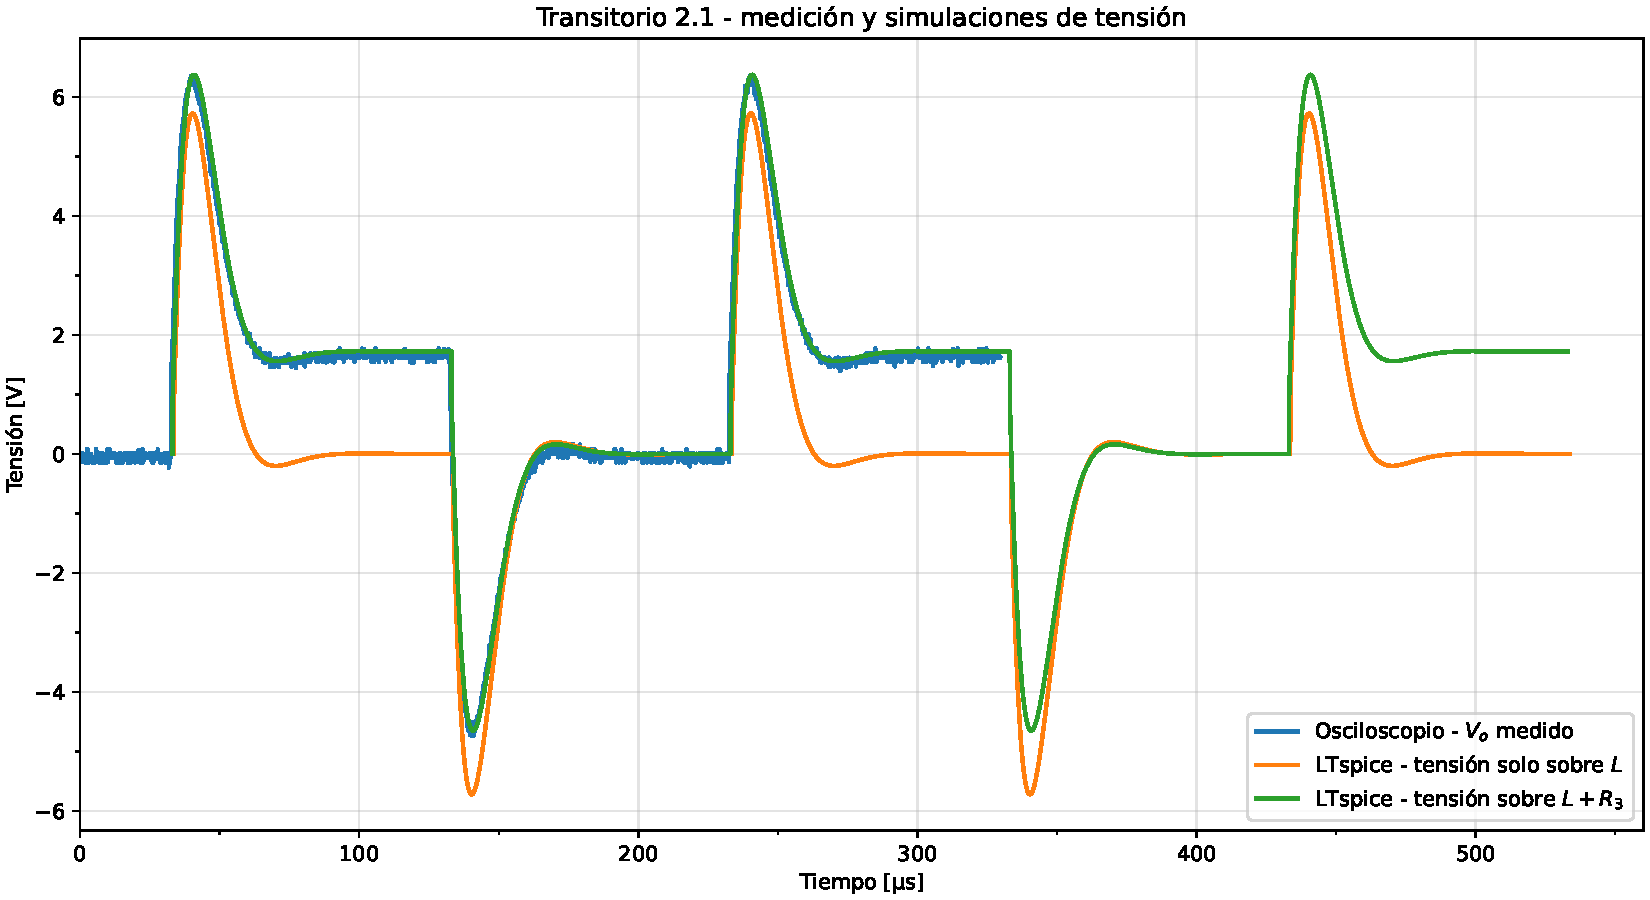
\includegraphics[width=0.94\textwidth,height=0.70\textheight,keepaspectratio]{transitorio_2_1_tensiones_comparacion_alineado.pdf}
    \smallnote{Las curvas se alinearon temporalmente para comparar la forma del transitorio y el sobrepico.}
\end{frame}

\begin{frame}{Corriente simulada en el capacitor}
    \centering
    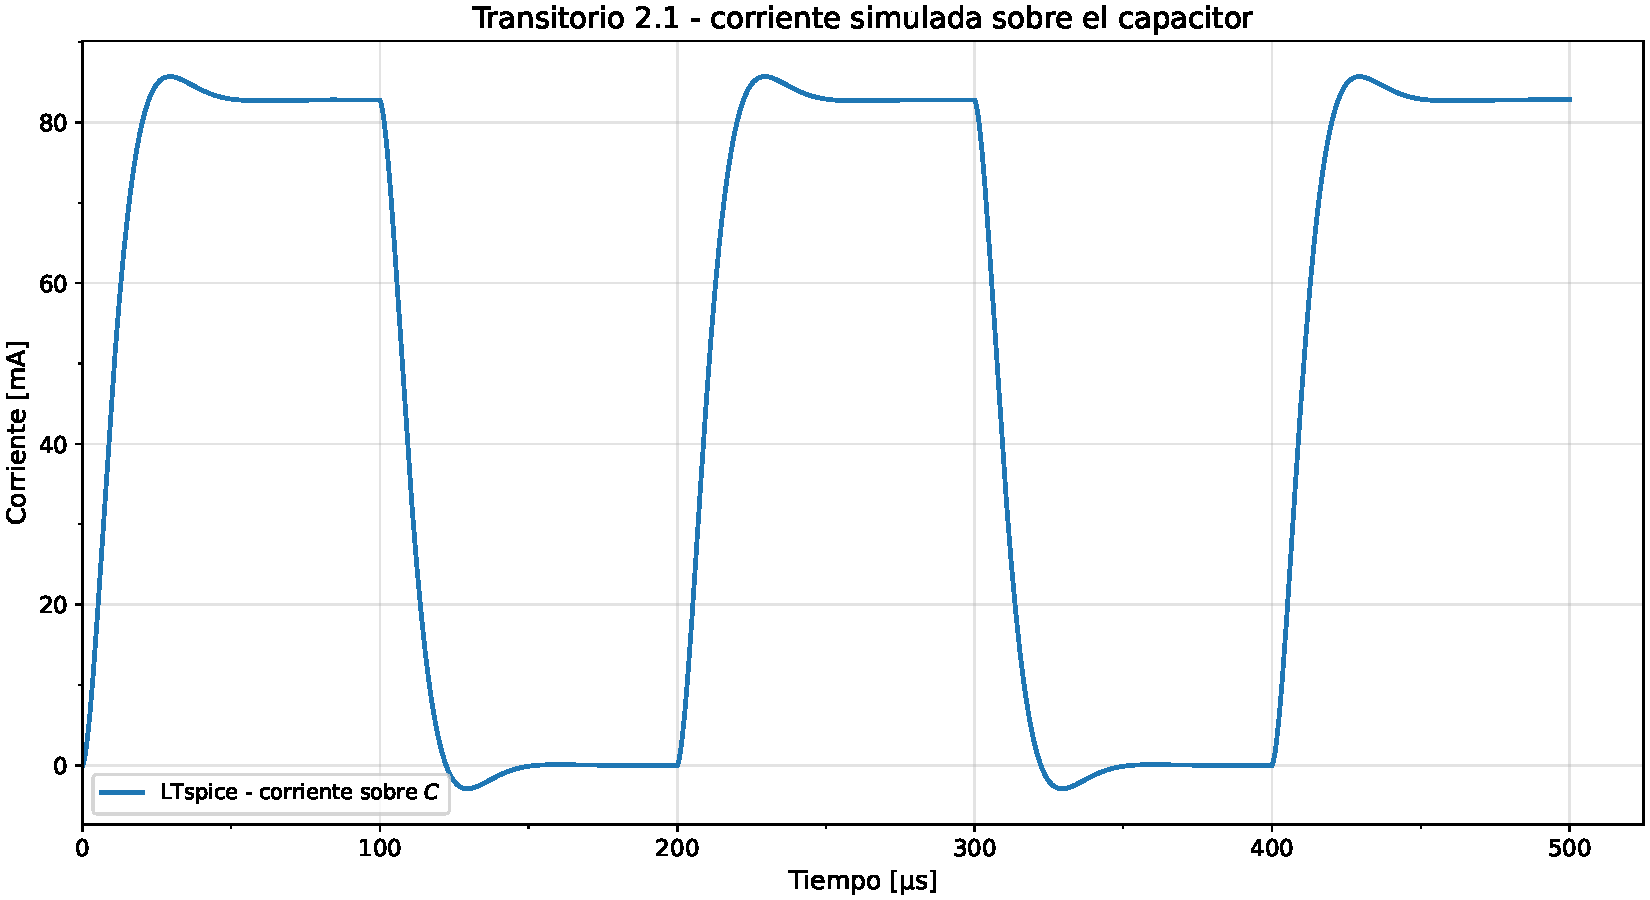
\includegraphics[width=0.92\textwidth,height=0.70\textheight,keepaspectratio]{transitorio_2_1_corriente_capacitor_simulada.pdf}
    \smallnote{La corriente presenta los picos esperados durante los cambios de estado de la llave.}
\end{frame}

\begin{frame}{Pseudofrecuencia y sobrepico}
    \begin{columns}[T,onlytextwidth]
        \column{0.50\textwidth}
        \centering
        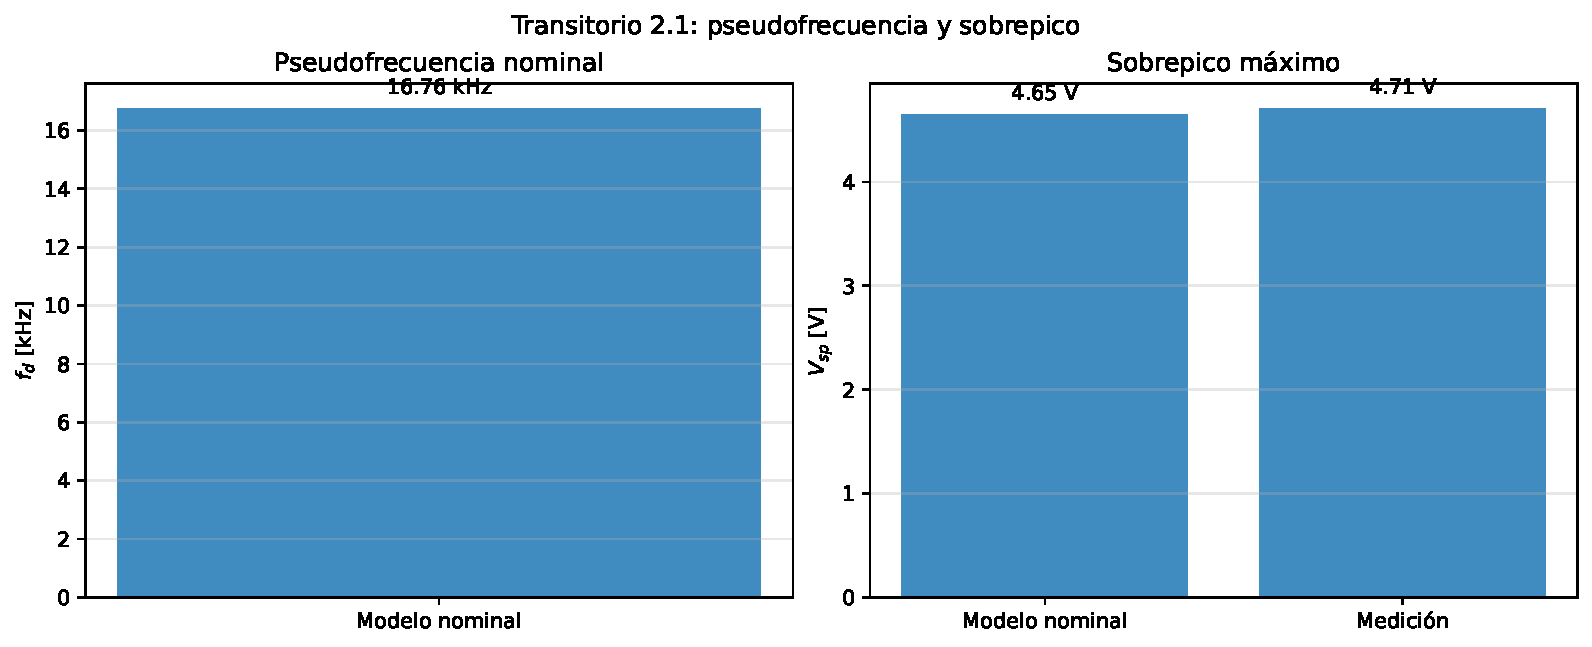
\includegraphics[width=\textwidth,height=0.63\textheight,keepaspectratio]{transitorio_21_pseudofrecuencia_sobrepico.pdf}
        \column{0.46\textwidth}
        \begin{block}{Parámetros usados}
        \begin{equation*}
            f_d=\frac{\omega_d}{2\pi}
        \end{equation*}
        \begin{equation*}
            V_{sp}=V_{max}-V_{final}
        \end{equation*}
        \end{block}
        \begin{itemize}
            \item $f_d$ mide la oscilación amortiguada.
            \item El sobrepico resume cuánto excede el valor final.
            \item Las diferencias provienen de tolerancias, resistencias parásitas y el armado real.
        \end{itemize}
    \end{columns}
\end{frame}

\begin{frame}{Montecarlo del transitorio}
    \begin{columns}[T,onlytextwidth]
        \column{0.50\textwidth}
        \centering
        
\includegraphics[width=\textwidth,height=0.62\textheight,keepaspectratio]{montecarlo_transitorio_21_histogramas.pdf}
        \column{0.46\textwidth}
        \begin{block}{Tolerancias}
        \begin{itemize}
            \item Resistencias: $5\%$.
            \item Capacitor: $10\%$.
            \item Inductor: $0\%$.
        \end{itemize}
        \end{block}
        \begin{itemize}
            \item Variar $C$ desplaza principalmente la frecuencia.
            \item Variar $R_2$ y $R_3$ modifica el amortiguamiento y el sobrepico.
            \item Con resistencias nulas se obtiene un caso ideal no realizable por pérdidas parásitas.
        \end{itemize}
    \end{columns}
\end{frame}

% -----------------------------------------------------------------
\section{Filtros de segundo orden}

\begin{frame}{Parámetros comunes de los RLC}
    \begin{columns}[T,onlytextwidth]
        \column{0.48\textwidth}
        \begin{block}{Ecuación característica}
        \begin{equation*}
            s^2LC+sRC+1=0
        \end{equation*}
        \begin{equation*}
            \omega_0=\frac{1}{\sqrt{LC}},\qquad Q=\frac{\omega_0 L}{R}
        \end{equation*}
        \end{block}
        \column{0.48\textwidth}
        \begin{block}{Con $R=50\Omega$, $L=1$mH, $C=82$nF}
        \begin{align*}
            f_0&\approx \SI{17.6}{kHz}\\
            Q&\approx 2.21\\
            B&\approx \SI{7.96}{kHz}
        \end{align*}
        \end{block}
        \begin{equation*}
            \omega_{1,2}=\mp\alpha+\sqrt{\alpha^2+\omega_0^2},\quad \alpha=\frac{R}{2L}
        \end{equation*}
    \end{columns}
\end{frame}

\begin{frame}{Circuitos analizados y tipo de filtro}
    \begin{center}
    \begin{tabular}{clc}
        \toprule
        Circuito & Salida tomada sobre & Tipo \\
        \midrule
        2 & Capacitor & Pasabajos \\
        3 & Inductor & Pasaaltos \\
        4 & Resistencia & Pasabanda \\
        5 & Conjunto $L+C$ & Rechazo de banda \\
        \bottomrule
    \end{tabular}
    \end{center}
    \vspace{0.8em}
    \begin{columns}[T,onlytextwidth]
        \column{0.48\textwidth}
        \begin{equation*}
            H_2(s)=\frac{1}{s^2LC+sRC+1}
        \end{equation*}
        \begin{equation*}
            H_3(s)=\frac{s^2LC}{s^2LC+sRC+1}
        \end{equation*}
        \column{0.48\textwidth}
        \begin{equation*}
            H_4(s)=\frac{sRC}{s^2LC+sRC+1}
        \end{equation*}
        \begin{equation*}
            H_5(s)=\frac{s^2LC+1}{s^2LC+sRC+1}
        \end{equation*}
    \end{columns}
\end{frame}

\begin{frame}{Respuesta teórica y fase}
    \begin{columns}[T,onlytextwidth]
        \column{0.49\textwidth}
        \centering
        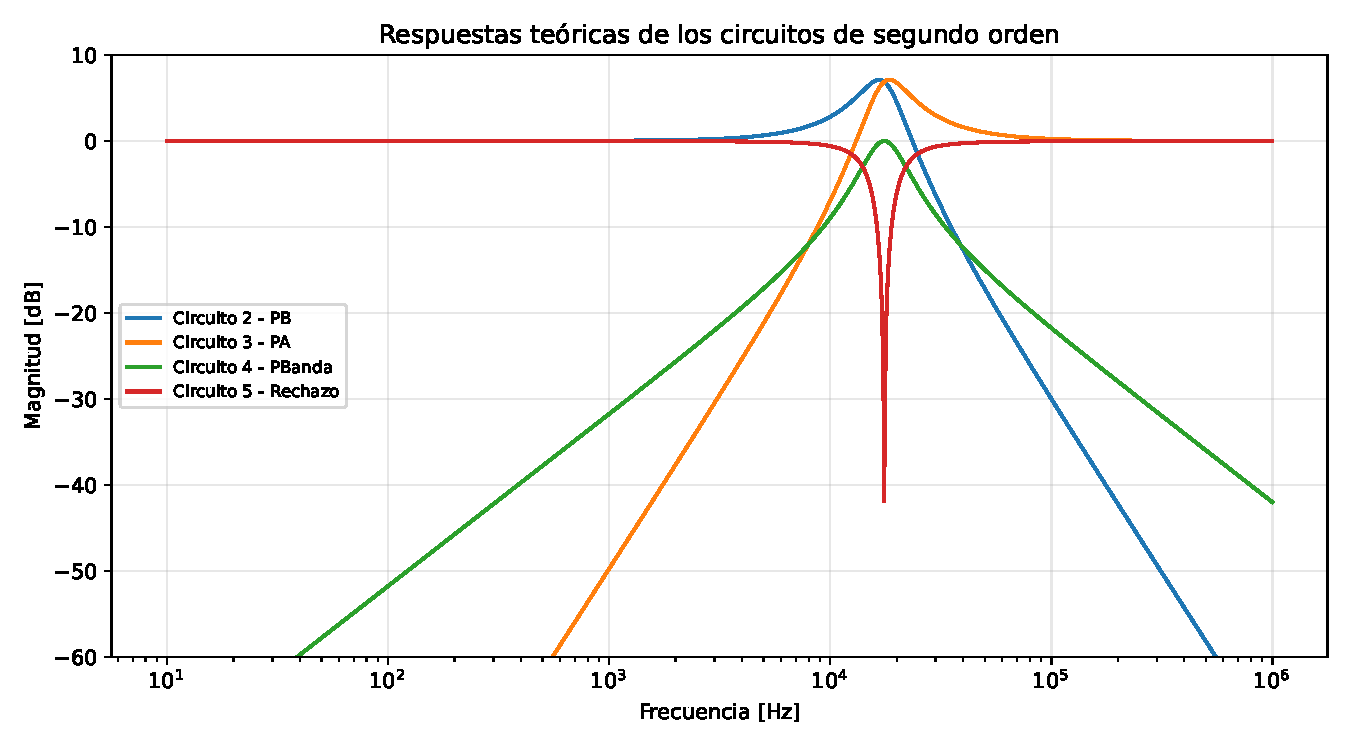
\includegraphics[width=\textwidth,height=0.62\textheight,keepaspectratio]{bode_filtros_teoricos.pdf}
        \column{0.49\textwidth}
        \centering
        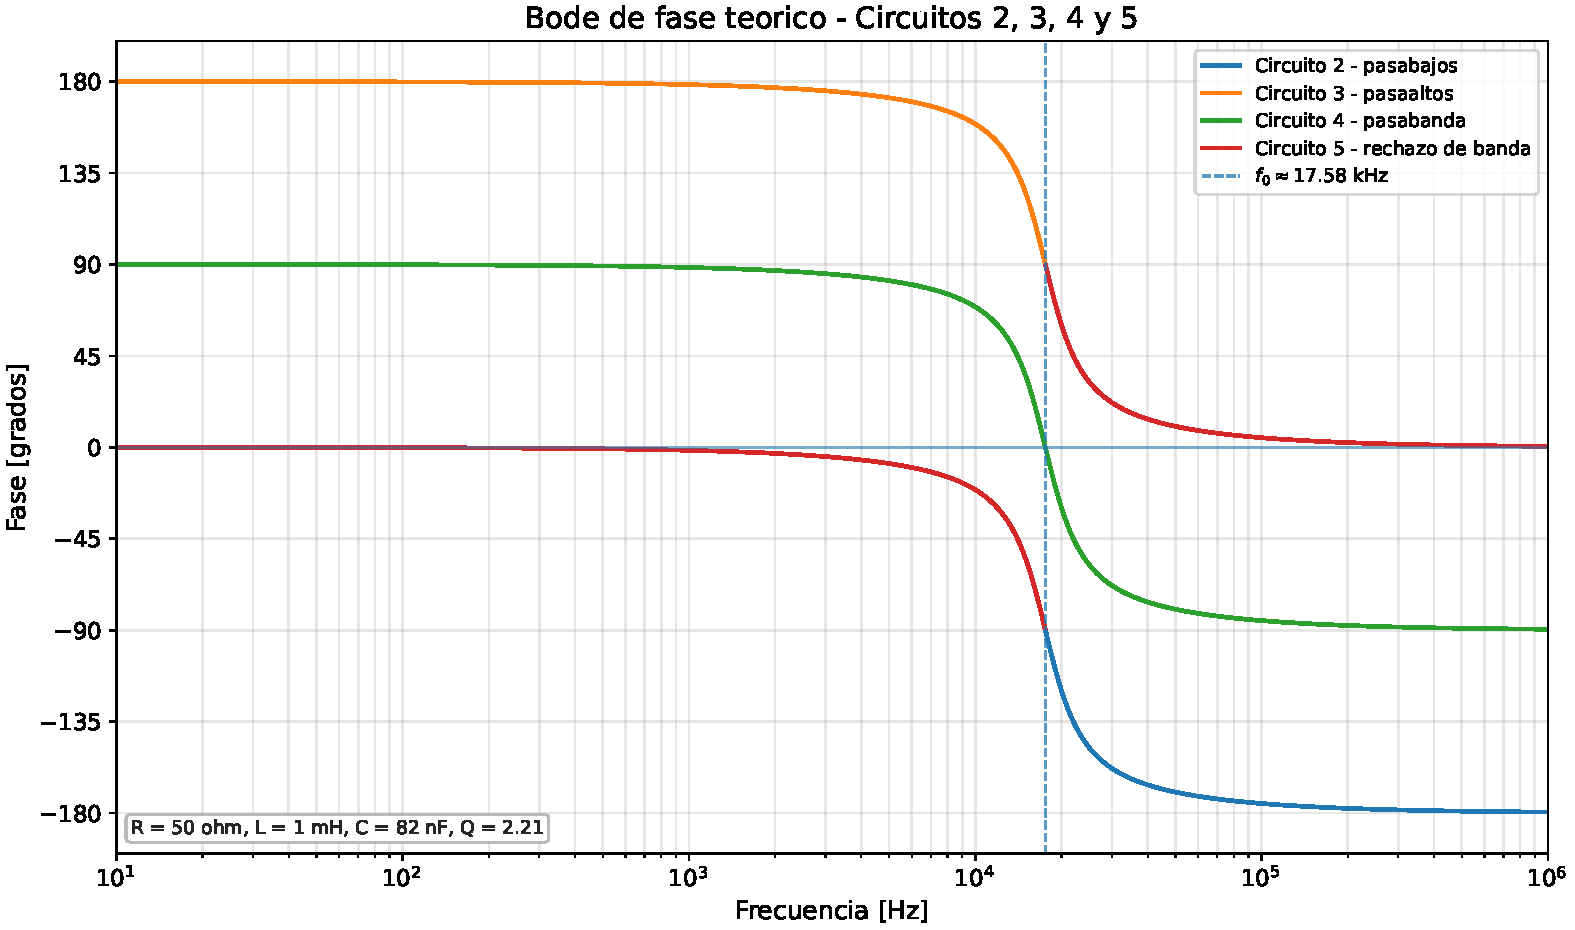
\includegraphics[width=\textwidth,height=0.62\textheight,keepaspectratio]{bode_fase_circuitos_2_3_4_5.pdf}
    \end{columns}
    \smallnote{Los cuatro circuitos comparten polos; cambia el numerador y, por lo tanto, los ceros.}
\end{frame}

\begin{frame}{Polos y ceros}
    \centering
    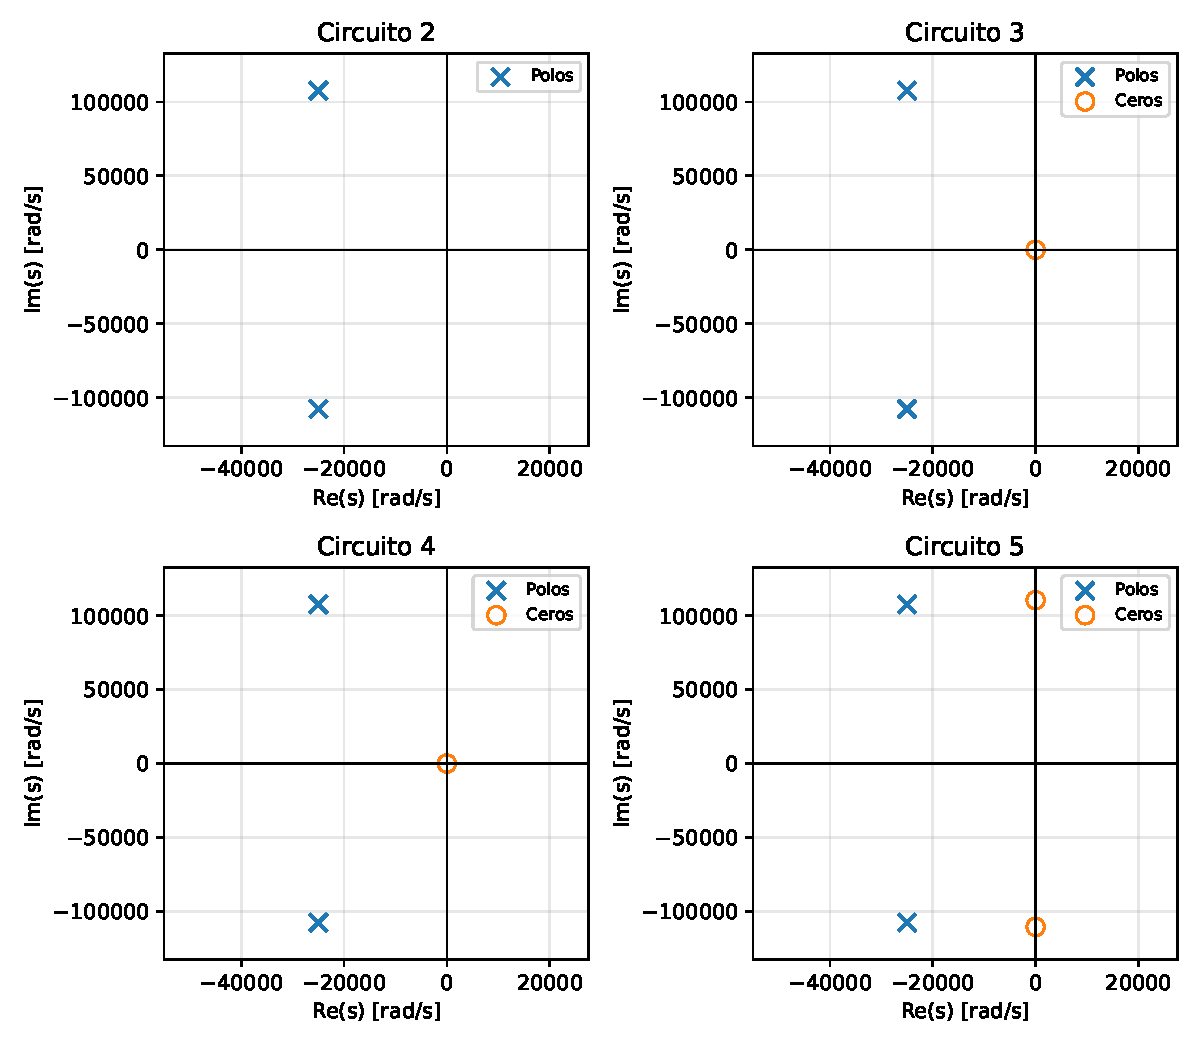
\includegraphics[width=0.88\textwidth,height=0.70\textheight,keepaspectratio]{polos_ceros_circuitos.pdf}
    \smallnote{Pasabajos: sin ceros finitos. Pasaaltos: dos ceros en el origen. Pasabanda: un cero en el origen. Rechazo: ceros en $\pm j\omega_0$.}
\end{frame}

\begin{frame}{Circuitos 2 y 5: medición vs simulación}
    \begin{columns}[T,onlytextwidth]
        \column{0.49\textwidth}
        \centering
        
\includegraphics[width=\textwidth,height=0.62\textheight,keepaspectratio]{bode_circuito2.pdf}
        \column{0.49\textwidth}
        \centering
        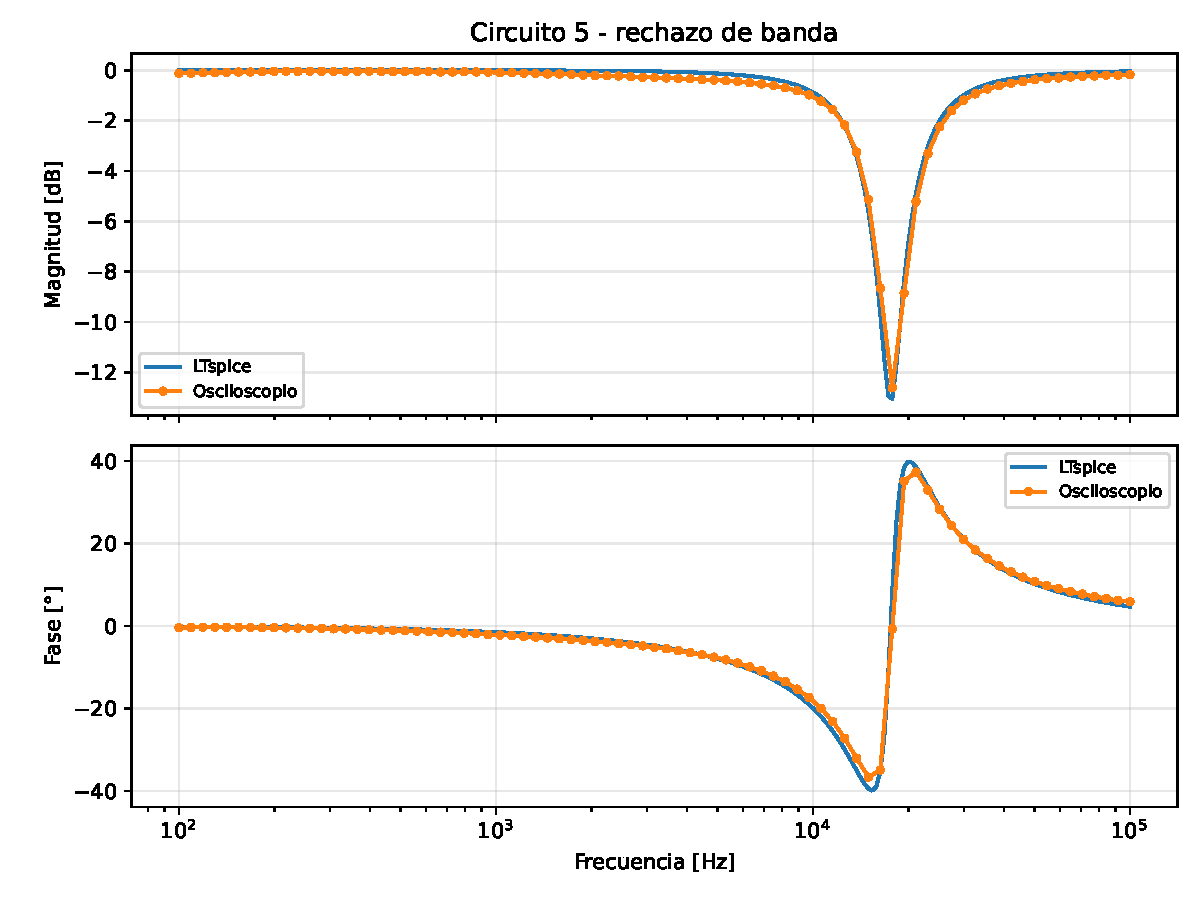
\includegraphics[width=\textwidth,height=0.62\textheight,keepaspectratio]{bode_circuito5.pdf}
    \end{columns}
    \smallnote{Las diferencias se explican por resistencia serie de la bobina, tolerancias y contactos de protoboard.}
\end{frame}

\begin{frame}{Montecarlo del Circuito 5}
    \begin{columns}[T,onlytextwidth]
        \column{0.56\textwidth}
        \centering
        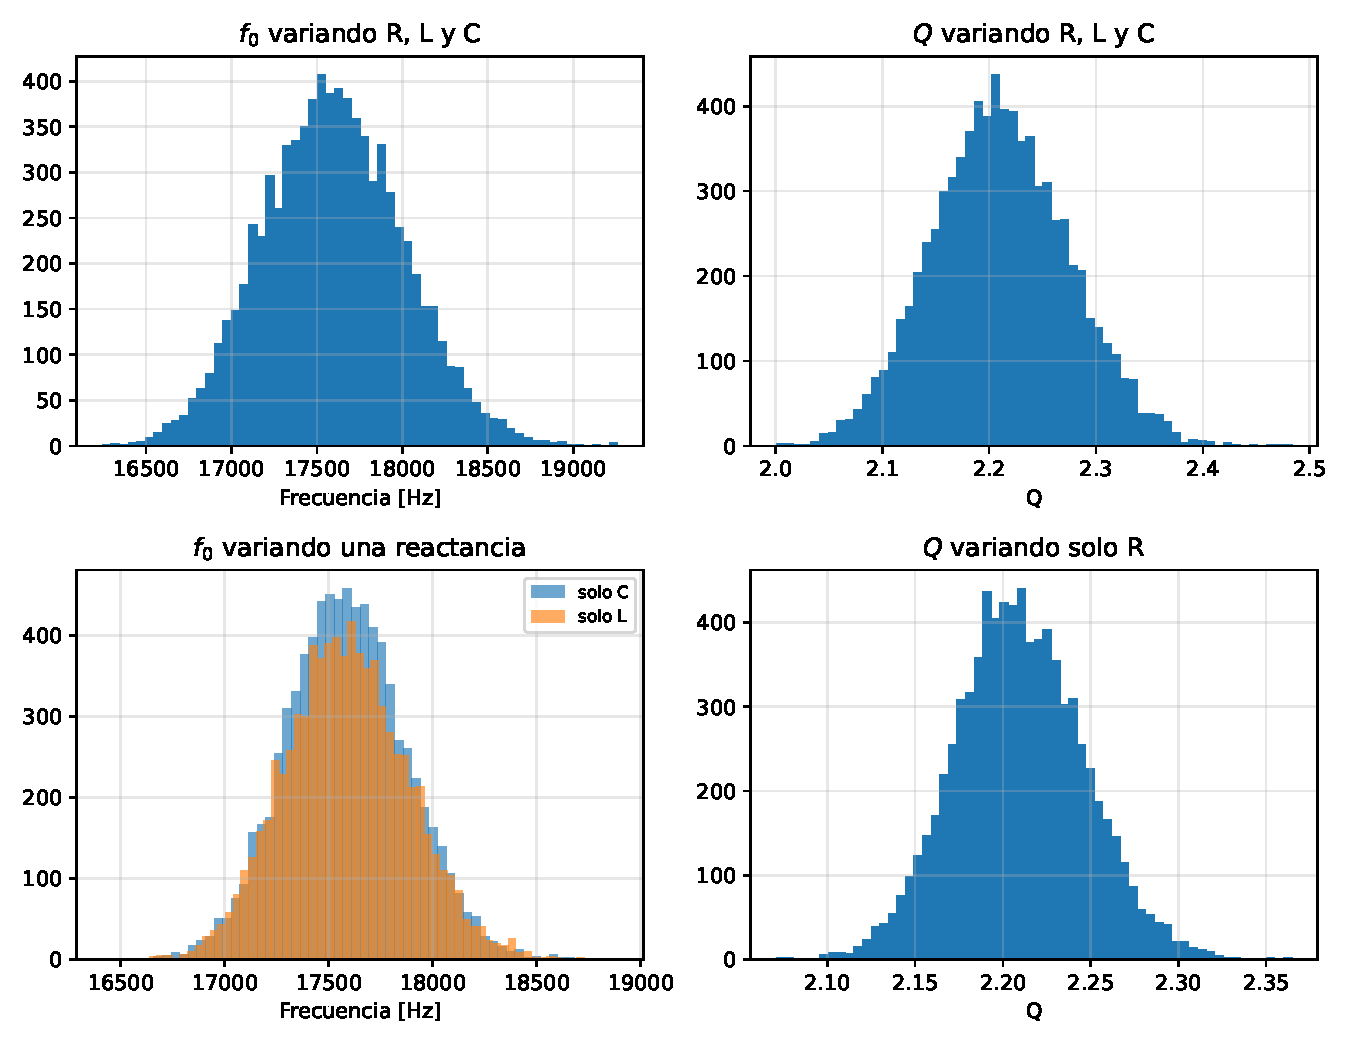
\includegraphics[width=\textwidth,height=0.65\textheight,keepaspectratio]{montecarlo_circuito5.pdf}
        \column{0.40\textwidth}
        \begin{itemize}
            \item Variar $L$ o $C$ desplaza $f_0$.
            \item Variar $R$ modifica el $Q$ y el ancho del rechazo.
            \item El resultado confirma la sensibilidad esperada:
        \end{itemize}
        \begin{equation*}
            f_0=\frac{1}{2\pi\sqrt{LC}},\qquad Q=\frac{1}{R}\sqrt{\frac{L}{C}}
        \end{equation*}
    \end{columns}
\end{frame}

% -----------------------------------------------------------------
\section{Filtro pasabanda para voz}

\begin{frame}{Especificación del producto}
    \begin{columns}[T,onlytextwidth]
        \column{0.50\textwidth}
        \begin{block}{Objetivo}
        Primer filtrado de voz humana con dos etapas y TL082 usado solo como buffer/no inversor.
        \end{block}
        \begin{equation*}
            \SI{300}{Hz}\lesssim f \lesssim \SI{3.4}{kHz}
        \end{equation*}
        \column{0.46\textwidth}
        \begin{itemize}
            \item Atenuar ruido de muy baja frecuencia.
            \item Atenuar contenido por encima de la banda de inteligibilidad.
            \item Mantener menos de \SI{3}{dB} de atenuación en banda útil.
        \end{itemize}
    \end{columns}
\end{frame}

\begin{frame}{Alternativas evaluadas}
    \begin{columns}[T,onlytextwidth]
        \column{0.52\textwidth}
        \centering
        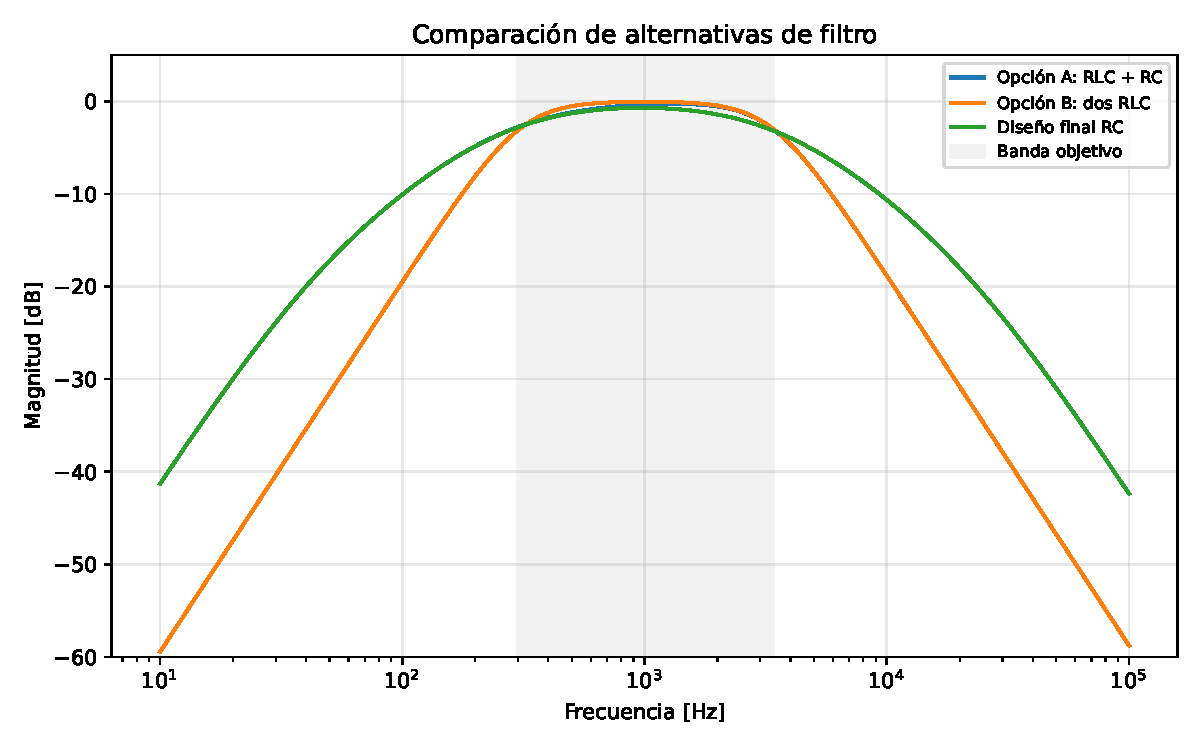
\includegraphics[width=\textwidth,height=0.58\textheight,keepaspectratio]{comparacion_opciones_filtro.pdf}
        \column{0.44\textwidth}
        \begin{block}{Descartes principales}
        \begin{itemize}
            \item RLC + RC-RC: respuesta poco simétrica entre etapas.
            \item Dos RLC con $L=1$mH: resistencia muy baja y corriente alta.
        \end{itemize}
        \end{block}
        \begin{alertblock}{Verificación}
        En simulación se obtuvo una corriente del orden de \SI{27}{mA} exigida al TL082.
        \end{alertblock}
    \end{columns}
\end{frame}

\begin{frame}{Diseño final adoptado}
    \centering
    \begin{adjustbox}{max width=0.96\textwidth}
    \begin{circuitikz}[american, scale=0.85, transform shape]
        \draw (0,0) node[left]{$v_i$} to[R,l=$R_1$] (2,0) coordinate(n1) to[R,l=$R_2$] (4,0) coordinate(n2);
        \draw (n1) to[C,l_=$C_1$] ++(0,-1.6) node[ground]{};
        \draw (n2) to[C,l_=$C_2$] ++(0,-1.6) node[ground]{};
        \node[op amp, noinv input up] (op1) at (5.8,0) {};
        \draw (n2) -- (op1.+);
        \draw (op1.out) -- ++(0.7,0) coordinate(b1);
        \draw (op1.-) -- ++(-0.3,0) |- (op1.out);
        \draw (b1) to[C,l=$C_3$] ++(1.8,0) coordinate(n3) to[C,l=$C_4$] ++(1.8,0) coordinate(n4);
        \draw (n3) to[R,l_=$R_3$] ++(0,-1.6) node[ground]{};
        \draw (n4) to[R,l_=$R_4$] ++(0,-1.6) node[ground]{};
        \node[op amp, noinv input up] (op2) at (12.2,0) {};
        \draw (n4) -- (op2.+);
        \draw (op2.out) -- ++(0.7,0) node[right]{$v_o$};
        \draw (op2.-) -- ++(-0.3,0) |- (op2.out);
    \end{circuitikz}
    \end{adjustbox}
    \vspace{0.8em}
    \begin{columns}[T,onlytextwidth]
        \column{0.48\textwidth}
        \begin{equation*}
            \Hpb(s)=\frac{1}{(sRC)^2+3sRC+1}
        \end{equation*}
        \column{0.48\textwidth}
        \begin{equation*}
            \Hpa(s)=\frac{(sRC)^2}{(sRC)^2+3sRC+1}
        \end{equation*}
    \end{columns}
\end{frame}

\begin{frame}{Valores del filtro final}
    \begin{columns}[T,onlytextwidth]
        \column{0.48\textwidth}
        \begin{block}{Pasabajos}
        \begin{align*}
            R_1=R_2&=\SI{1.8}{k\ohm}\\
            C_1=C_2&=\SI{10}{nF}
        \end{align*}
        \end{block}
        \begin{equation*}
            f_{c,PB}\approx 0.374\frac{1}{2\pi RC}
        \end{equation*}
        \column{0.48\textwidth}
        \begin{block}{Pasaaltos}
        \begin{align*}
            R_3=R_4&=\SI{15}{k\ohm}\\
            C_3=C_4&=\SI{100}{nF}
        \end{align*}
        \end{block}
        \begin{equation*}
            f_{c,PA}\approx 2.67\frac{1}{2\pi RC}
        \end{equation*}
    \end{columns}
    \vspace{0.5em}
    \begin{center}
        \large $H(s)=\Hpb(s)\,\Hpa(s)$
    \end{center}
\end{frame}

\begin{frame}{Implementación en Altium}
    \begin{columns}[T,onlytextwidth]
        \column{0.60\textwidth}
        \centering
        
\includegraphics[width=\textwidth,height=0.68\textheight,keepaspectratio]{esquematico_altium.png}
        \column{0.36\textwidth}
        \begin{itemize}
            \item Entrada por jack de audio y por conector.
            \item Selección de entrada.
            \item Alimentación simétrica $\pm\SI{12}{V}$.
            \item TL082 como seguidores de tensión.
            \item Salida por conector.
        \end{itemize}
    \end{columns}
\end{frame}

\begin{frame}{Bode del filtro final}
    \centering
    
\includegraphics[width=0.92\textwidth,height=0.70\textheight,keepaspectratio]{bode_filtro_final.pdf}
    \smallnote{La respuesta final se compara entre simulación y medición para verificar si cumple la banda de voz.}
\end{frame}

% -----------------------------------------------------------------
\section{Cierre}

\begin{frame}{Conclusiones}
    \begin{itemize}
        \item La GUI permitió una comparación rápida entre datos de osciloscopio, simulación y Bode.
        \item El transitorio mostró el comportamiento subamortiguado esperado y se cuantificaron $f_d$ y sobrepico.
        \item Los filtros RLC se clasificaron correctamente a partir de sus ceros y polos.
        \item Para el diseño de PCB se descartaron alternativas que no eran convenientes físicamente.
        \item La solución final RC-RC con buffers cumple la restricción de uso del TL082 y es realizable en PCB.
    \end{itemize}
    \vfill
    \begin{center}
        \Large \textbf{Preguntas}
    \end{center}
\end{frame}

\end{document}
